\documentclass{article}
\usepackage{graphicx}
\usepackage{float}
\usepackage{amsmath, amssymb, amsfonts}
\usepackage{siunitx}
\usepackage{circuitikz}
\usepackage{tikz}
\usepackage{xcolor}
\usepackage{hyperref}
\usepackage[a4paper, margin=1in]{geometry}
\usepackage{fancyhdr}

% Header Configuration
\pagestyle{fancy} 
\fancyhf{} % Clear default header/footer
\fancyhead[L]{\thesection. \nouppercase{\leftmark}} % Left-align: Section number & title
\fancyhead[R]{\thepage} % Right-align: Page number
\renewcommand{\headrulewidth}{0.4pt} % Line under the header
\renewcommand{\sectionmark}[1]{\markboth{#1}{}}

% Remove header from the first page
\thispagestyle{plain}

\title{ECE/CS 252: Intro to Computer Engineering}
\author{Kiplimo Kemei}
\date{Spring 2024}

\begin{document}

\maketitle

\section{Number Systems}
Binary: $\mathtt{1011_2}$, Octal: $\mathtt{35_8}$, Hexadecimal: $\mathtt{A3F_{16}}$

\section{Logic Gates}
\begin{circuitikz}
    \draw (0,0) node[nand port] (nand1) {};
\end{circuitikz}

\section{Boolean Algebra}
\[
    A + (B \cdot C) = (A + B) \cdot (A + C)
\]

\section{Figures and Images}
\begin{figure}[H]
    \centering
    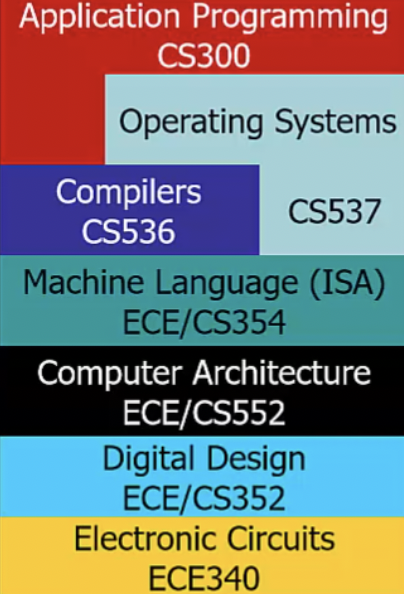
\includegraphics[width=0.5\textwidth]{image.png}
    \caption{Example Image}
\end{figure}

\end{document}